% Use only LaTeX2e, calling the article.cls class and 12-point type.

\documentclass[12pt]{article}


% Users of the {thebibliography} environment or BibTeX should use the
% scicite.sty package, downloadable from *Science* at
% www.sciencemag.org/about/authors/prep/TeX_help/ .
% This package should properly format in-text
% reference calls and reference-list numbers.

\usepackage{scicite}

% Use times if you have the font installed; otherwise, comment out the
% following line.

\usepackage{times}
\usepackage{graphicx}

% The preamble here sets up a lot of new/revised commands and
% environments.  It's annoying, but please do *not* try to strip these
% out into a separate .sty file (which could lead to the loss of some
% information when we convert the file to other formats).  Instead, keep
% them in the preamble of your main LaTeX source file.


% The following parameters seem to provide a reasonable page setup.
\topmargin 0.0cm
\oddsidemargin 0.2cm
\textwidth 16cm 
\textheight 21cm
\footskip 1.0cm


%The next command sets up an environment for the abstract to your paper.

\newenvironment{sciabstract}{%
\begin{quote} \bf}
{\end{quote}}


% If your reference list includes text notes as well as references,
% include the following line; otherwise, comment it out.

\renewcommand\refname{References and Notes}

% The following lines set up an environment for the last note in the
% reference list, which commonly includes acknowledgments of funding,
% help, etc.  It's intended for users of BibTeX or the {thebibliography}
% environment.  Users who are hand-coding their references at the end
% using a list environment such as {enumerate} can simply add another
% item at the end, and it will be numbered automatically.

\newcounter{lastnote}
\newenvironment{scilastnote}{%
\setcounter{lastnote}{\value{enumiv}}%
\addtocounter{lastnote}{+1}%
\begin{list}%
{\arabic{lastnote}.}
{\setlength{\leftmargin}{.22in}}
{\setlength{\labelsep}{.5em}}}
{\end{list}}


% Include your paper's title here

\title{The length of words reflects their conceptual complexity}


% Place the author information here.  Please hand-code the contact
% information and notecalls; do *not* use \footnote commands.  Let the
% author contact information appear immediately below the author names
% as shown.  We would also prefer that you don't change the type-size
% settings shown here.

\author
{Molly Lewis and Michael C. Frank\\
\\
\normalsize{Psychology Department, Stanford University,}\\
\normalsize{450 Serra Mall, Stanford, CA 94305, USA}\\
\\
\normalsize{$^\ast$To whom correspondence should be addressed; E-mail: mll@stanford.edu.}
}


% Include the date command, but leave its argument blank.

\date{}



%%%%%%%%%%%%%%%%% END OF PREAMBLE %%%%%%%%%%%%%%%%
\begin{document} 

% Double-space the manuscript.
\baselineskip24pt

% Make the title.
\maketitle 

% Place your abstract within the special {sciabstract} environment.

\begin{sciabstract}
 Are the forms of words systematically related to their meaning? The �arbitrariness of the sign� has long been a foundational part of our understanding of human language\cite{saussure, hockett1960}. Theories of communication predict a relationship between form and meaning, however: longer descriptions should convey more complex meanings\cite{horn1984,jaeger2006}. Here we show that the lexicons of human languages reflect this relationship between linguistic and cognitive complexity. We asked participants to rate the conceptual complexity of word meanings and found that their judgements correlated highly with word length across XX languages, even controlling for frequency and concreteness. This relationship is productively encoded in the minds of speakers, as well: Adults and children both mapped longer words to more complex meanings, and more complex meanings to longer words, in comprehension and production tasks and across a wide range of stimuli. In addition, explicit judgments of complexity were highly correlated with an implicit measure of study time in a memory task, suggesting that complexity is directly related to basic cognitive processes. These results point to a general regularity in the design of lexicons and suggests the importance of cognitive constraints on language evolution\cite{christiansen2008,lieberman2007}.
 \end{sciabstract}


%Letters no more than 4 pages, of Nature. A typical Letter to Nature contains about 1,500 words of text (excluding the first paragraph of Letters, figure legends, reference list and the methods section if applicable) and four small display items (figures and/or tables) with brief legends. A composite figure (with several panels) usually needs to take about half a page, equivalent to about 600 words, in order for all the elements to be visible (see section 5.9 for instructions on sizing figures).

% intro
Human languages universally contain sequences of sounds --- words --- that are associated with particular meanings. A foundational part of our understanding of human language is that these associations are arbitrary \cite{saussure,hocket1960}. This assumption is supported by a superficial survey of word forms across languages: different languages use different words to refer to similar meanings.  However, several theories of communication predict a systematicity in these mappings\cite{horn1984,jaeger2006}.  They predict that longer utterances should be associated with more complex meanings (a complexity bias). Here we address whether this bias is present in language at the level of words. We first examine whether speakers have a lexical complexity bias that is productive by asking how speakers interpret novel words. Given evidence for a productive complexity bias in words, we then ask whether this systematicity is encoded in the lexicon of XX languages. 

%communicative pressures should lead to a complexity bias that operates at the moment of language interpretation.

%Uniform information theory predicts that  speakers should try to maintain a constant rate of information transfer across the speech stream. A straight forward consequence of this prediction is that speakers should try to use longer linguistic forms to refer to less predictable meanings.
%More specifically, they predict that com- municative pressures should lead to a complexity bias that op- erates at the moment of language interpretation.

%Uniform information theory predicts that  speakers should try to maintain a constant rate of information transfer across the speech stream. A straight forward consequence of this prediction is that speakers should try to use longer linguistic forms to refer to less predictable meanings. 

In Study 1, we asked whether speakers show a bias to map a relatively long novel word onto a relatively more complex referent. 
Participants were presented with 

From an information theoretic perspective, 

\begin{figure}[t]
\begin{center}
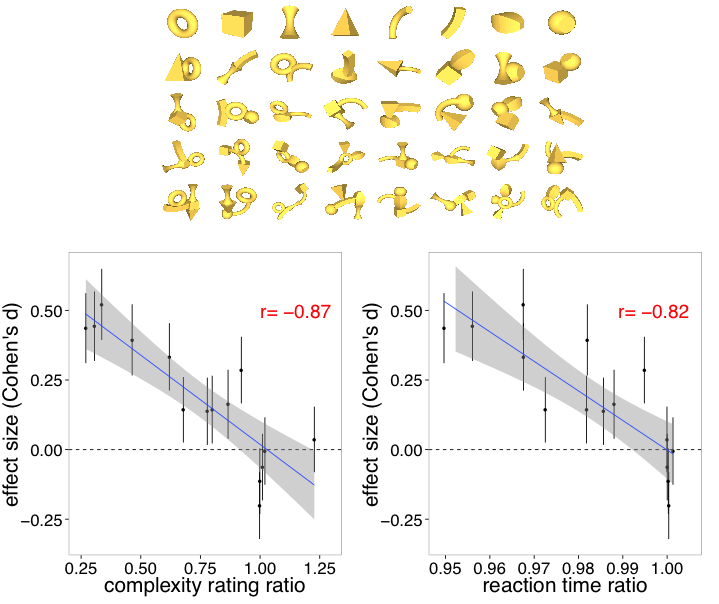
\includegraphics[scale = .5]{figs/geons_cropped.png}
\end{center}
\end{figure}

\begin{figure}[t]
\begin{center}
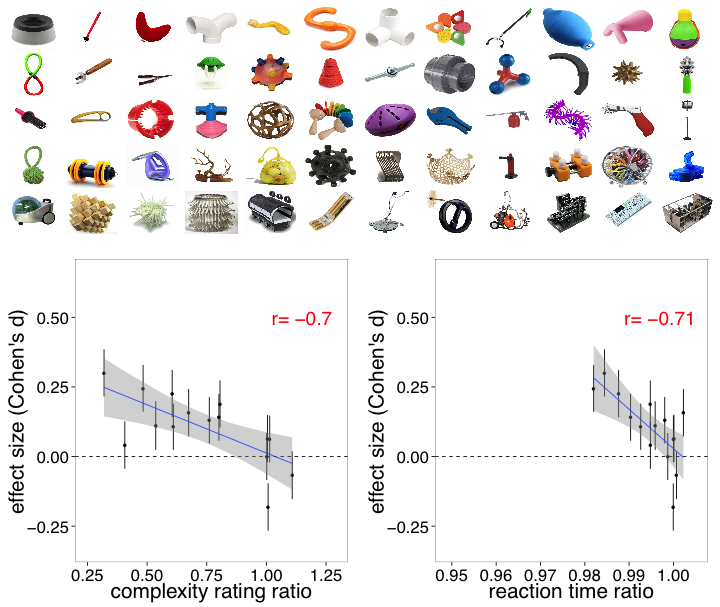
\includegraphics[scale = .5]{figs/real_objs_cropped.png}
\end{center}
\end{figure}




In Study 1, we asked whether speakers  norms + mapping

In Study 2, norms + mapping + production (a single sentence)

In Study , we did complexity norms. Highly correlated.

In Study 4, cross linguistic. 

Figs. 
(1) six panels with sorted display of images on left (geons + objects) and effect size plots on right (complexity + RT)
(2) bar graph of correlations (study 4) (with parial correlations, mono morphemic, and open class only)

% conclusion

\paragraph*{Tables}
\paragraph*{Figure Legends}
\paragraph*{Methods}
\paragraph*{References}
\paragraph*{Acknowledgements}
\paragraph*{Author Contributions}
\paragraph*{Author Information}


\bibliography{biblibrary}

\bibliographystyle{Science}



% Following is a new environment, {scilastnote}, that's defined in the
% preamble and that allows authors to add a reference at the end of the
% list that's not signaled in the text; such references are used in
% *Science* for acknowledgments of funding, help, etc.





% For your review copy (i.e., the file you initially send in for
% evaluation), you can use the {figure} environment and the
% \includegraphics command to stream your figures into the text, placing
% all figures at the end.  For the final, revised manuscript for
% acceptance and production, however, PostScript or other graphics
% should not be streamed into your compliled file.  Instead, set
% captions as simple paragraphs (with a \noindent tag), setting them
% off from the rest of the text with a \clearpage as shown  below, and
% submit figures as separate files according to the Art Department's
% instructions.


\clearpage



\end{document}



